\documentclass[border=1pt]{standalone}
\usepackage{newtxtext,newtxmath}
\usepackage{pgfplots}
\usetikzlibrary{calc}
\pgfplotsset{compat=1.18}
\definecolor{obs}{HTML}{D55E00}
\definecolor{sens}{HTML}{0072B2}
\begin{document}
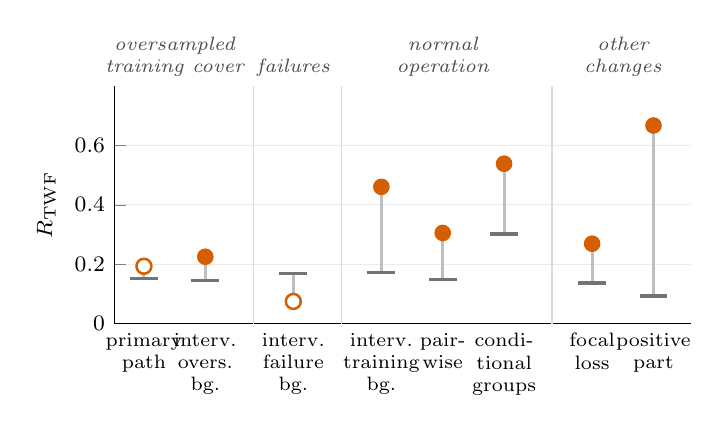
\begin{tikzpicture}[
  stick/.style={line width=1.1pt, black!25}, nullmark/.style={line width=1.3pt, black!55},
  aligned/.style={circle, fill=obs, draw=obs, line width=0.6pt, inner sep=0pt, minimum size=5.4pt},
  notaligned/.style={circle, fill=white, draw=obs, line width=0.9pt, inner sep=0pt, minimum size=5.4pt},
  sep/.style={black!14, line width=0.5pt}, head/.style={font=\scriptsize\itshape, align=center, anchor=south, text=black!70}]
\begin{axis}[width=8.9cm, height=4.6cm, xmin=-0.55, xmax=10.25, ymin=0, ymax=0.8,
  axis x line*=bottom, axis y line*=left, clip=false,
  xtick={0.00,1.15,2.80,4.45,5.60,6.75,8.40,9.55}, xticklabels={{primary\\path},{interv.\\overs.\\bg.},{interv.\\failure\\bg.},{interv.\\training\\bg.},{pair-\\wise},{condi-\\tional\\groups},{focal\\loss},{positive\\part}},
  xticklabel style={align=center, font=\scriptsize}, x tick style={draw=none},
  ytick={0,0.2,0.4,0.6}, yticklabel style={font=\footnotesize, /pgf/number format/fixed},
  ylabel={$R_{\mathrm{TWF}}$}, ylabel style={font=\footnotesize}, ymajorgrids, grid style={black!8}]
\draw[stick] (axis cs:0.0,0.1516) -- (axis cs:0.0,0.1934);
\draw[nullmark] (axis cs:-0.26,0.1516) -- (axis cs:0.26,0.1516);
\node[notaligned] at (axis cs:0.0,0.1934) {};
\draw[stick] (axis cs:1.15,0.1451) -- (axis cs:1.15,0.2253);
\draw[nullmark] (axis cs:0.8899999999999999,0.1451) -- (axis cs:1.41,0.1451);
\node[aligned] at (axis cs:1.15,0.2253) {};
\draw[stick] (axis cs:2.8,0.1688) -- (axis cs:2.8,0.0749);
\draw[nullmark] (axis cs:2.54,0.1688) -- (axis cs:3.0599999999999996,0.1688);
\node[notaligned] at (axis cs:2.8,0.0749) {};
\draw[stick] (axis cs:4.449999999999999,0.1717) -- (axis cs:4.449999999999999,0.4606);
\draw[nullmark] (axis cs:4.1899999999999995,0.1717) -- (axis cs:4.709999999999999,0.1717);
\node[aligned] at (axis cs:4.449999999999999,0.4606) {};
\draw[stick] (axis cs:5.6,0.1489) -- (axis cs:5.6,0.3054);
\draw[nullmark] (axis cs:5.34,0.1489) -- (axis cs:5.859999999999999,0.1489);
\node[aligned] at (axis cs:5.6,0.3054) {};
\draw[stick] (axis cs:6.75,0.3016) -- (axis cs:6.75,0.5385);
\draw[nullmark] (axis cs:6.49,0.3016) -- (axis cs:7.01,0.3016);
\node[aligned] at (axis cs:6.75,0.5385) {};
\draw[stick] (axis cs:8.4,0.1377) -- (axis cs:8.4,0.2693);
\draw[nullmark] (axis cs:8.14,0.1377) -- (axis cs:8.66,0.1377);
\node[aligned] at (axis cs:8.4,0.2693) {};
\draw[stick] (axis cs:9.55,0.0934) -- (axis cs:9.55,0.6672);
\draw[nullmark] (axis cs:9.290000000000001,0.0934) -- (axis cs:9.81,0.0934);
\node[aligned] at (axis cs:9.55,0.6672) {};
\draw[sep] (axis cs:2.05,0) -- (axis cs:2.05,0.8);
\draw[sep] (axis cs:3.6999999999999997,0) -- (axis cs:3.6999999999999997,0.8);
\draw[sep] (axis cs:7.65,0) -- (axis cs:7.65,0.8);
\node[head] at (axis cs:0.575,0.8) {oversampled\\training cover};
\node[head] at (axis cs:2.8,0.8) {failures};
\node[head] at (axis cs:5.6,0.8) {normal\\operation};
\node[head] at (axis cs:8.975000000000001,0.8) {other\\changes};
\end{axis}
\end{tikzpicture}
\end{document}
